Electron efficiencies are evaluated using the Tag-and-Probe method~\cite{CMS-EWK-10-005}.
The study was performed on the SingleElectron/EGamma dataset for each year separately.

Tag electrons need to satisfy the following quality requirements:
\begin{itemize}
\item trigger matched to single electron trigger;
\item $\pt > 30 \GeV$, supercluster (SC) $|\eta| < 2.17$;% but on in EB-EE gap ($1.4442<|\eta|<1.566$)
\item the tag and the probe need to have opposite charge.
%\item tight working point of the Spring16 cut-based electron ID
\end{itemize}

For the bin of probe \pt between 7 and 20\GeV, additional criteria are required:
\begin{itemize}
\item the tag has to pass a cut on the MVA score;
\item $\sqrt{2*\ptmiss*\pt^{tag}*(1-cos(\phi_{\rm MET}-\phi_{tag}))} < 45 \GeV$;
\item tag minimum \pt increased to 50\GeV;
\item the charge is determined with the so-called selection method, requiring that all three estimates of the electron charge agree.
\end{itemize}
These cuts help cleaning the background and make the fits more reliable (and thus, the measurement more precise).

Probe electrons only need to be reconstructed with the Gaussian sum filter, while the FSR recovery algorithm is not applied.

The nominal simulation efficiencies are evaluated from the a Drell-Yan sample simulated with \MADGRAPH at Leading Order in QCD,
using a template fit.
The $m_{ee}$ signal shape of the passing and failing probes are taken from MC and convoluted with a Gaussian.
The data is then fitted with the convoluted MC templates and a CMSShape (an Error-function with a one-sided exponential tail).
For the low \pt bins, a Gaussian is added to the signal model for the failing probes.

%\paragraph{Electron selection efficiency measurements}\mbox{}\\
%\label{par:Efficiency_measurements}

The electron selection efficiency is measured as a function of the probe electron $p_{T}$ and its SC $\eta$, and separately for electrons falling in the ECAL gaps.

%Figure \ref{fig:ele_sel_pt_turn_onA},~\ref{fig:ele_sel_pt_turn_onB},~\ref{fig:ele_sel_pt_turn_onC} and~\ref{fig:ele_ele_eta_turn_onA},\ref{fig:ele_ele_eta_turn_onB},~\ref{fig:ele_ele_eta_turn_onC} show the $p_{T}$ and $\eta$ turn-on curves measured in data, for 2016, 2017 and 2018.
% and the final 2D scale factor is shown in Fig.~\ref{fig:ele_sel_scale_factors} together with the systematic uncertainties. %These scale factors are very similar to the ICHEP figures, but more homogenous across $\eta$ and $p_{T}$ because of the higher statistics and the usage of more stable fitting routines in the new T\&P tool.

%\includegraphics[page=2, width=0.4\textwidth]{Figures/Electrons/ErecoEta}\\

Standard practices for the evaluation of Tag-and-Probe uncertainties for efficiency measurements are followed. Specifically, the following were considered:

\begin{itemize}
   \item Variation of the signal shape from the MC shape to an analytic shape (Crystal Ball) fitted to the MC
   \item Variation of the background shape from a CMS-shape to a simple exponential in fits to data
   \item Using an NLO MC sample for the signal templates
\end{itemize}

The total uncertainty for the measurement of the scale factors is the quadratic sum of the statistical uncertainties returned from the fit and the aforementioned systematic uncertainties.

The resulting efficiencies and corresponding scale factors, expressed as ratio of the efficiency observed in data to that calculated in simulation are reported
in Figure~\ref{fig:eleMVAEffSF}.

\begin{figure}
\centering
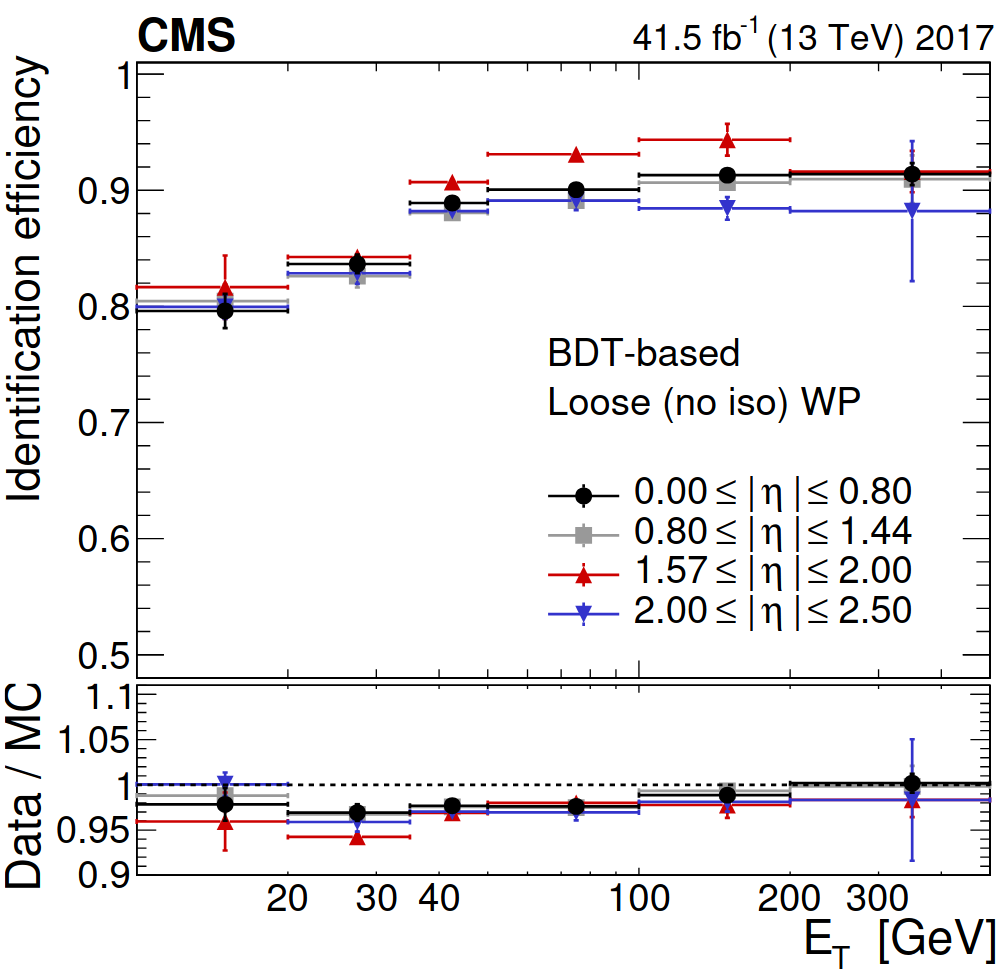
\includegraphics[width=.5\textwidth]{eleMVAEffSF2017.png}
\caption{Electron selection efficiencies in data (upper panel)
  and data-to-simulation ratio (lower panel),
  measured using the Tag-and-Probe technique
  as a function of the transverse energy}
\label{fig:eleMVAEffSF}
\end{figure}

